\chapter{相关理论和技术介绍}

\section{大语言模型概述}

大语言模型（Large Language Models，LLM）是近年来自然语言处理领域最具代表性的技术进展之一。其基本思路是通过大规模文本训练，让模型学习语言中的语法规律、语义关系和上下文依赖。与传统模型相比，大语言模型参数规模更大，能够处理更复杂的语言现象，也因此在问答、对话、摘要和内容生成等任务中表现出更强的泛化能力。当前主流大语言模型大多建立在Transformer框架之上，因此理解Transformer的基本原理，是分析后续RAG系统与模型优化方法的前提。

\subsection{Transformer模型}

Transformer由Vaswani等人在2017年提出\cite{Vaswani_2017_AttentionIsAllYouNeed}，其关键突破在于用自注意力机制替代传统循环结构建模序列关系。与RNN和LSTM相比，Transformer不需要按时间步逐次处理输入，因此训练并行度更高，也更容易捕捉长距离依赖关系。这两个特点直接推动了其在大规模预训练中的广泛应用。

\begin{figure}[htb]
    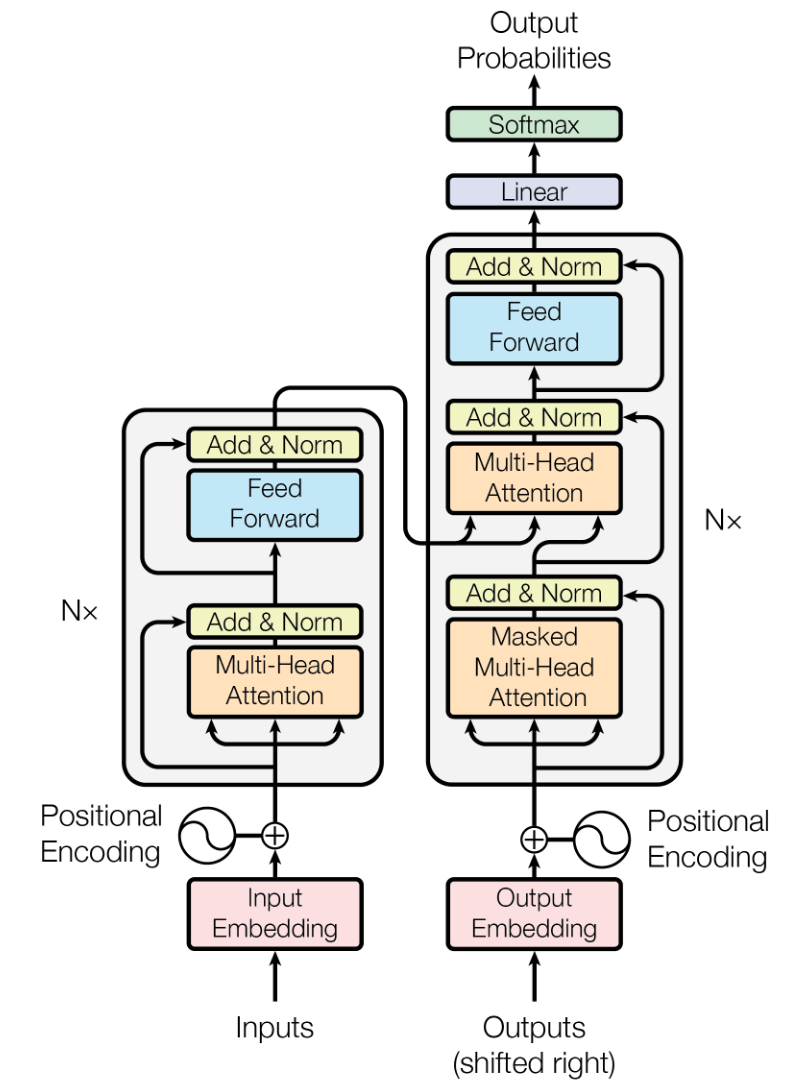
\includegraphics[width=0.5 \textwidth]{image/2/transformer1.png}
    \caption{Transformer结构图}
    \label{fig:transformer-structure}
\end{figure}

如图\ref{fig:transformer-structure}所示，Transformer由编码器和解码器两部分组成。编码器负责将输入序列转换为高维语义表示，解码器则依据这些表示逐步生成输出。编码器和解码器都由多层重复堆叠构成，其中最核心的模块是多头自注意力和前馈神经网络。为了提升训练稳定性，模型还在各子层后加入残差连接和归一化操作。解码器与编码器相比，多了掩码自注意力和编码器-解码器注意力，用于保证生成过程满足自回归约束，并充分利用输入语义信息。

自注意力机制是Transformer的核心。它的作用不是简单地“看上下文”，而是根据当前词与序列中其他词之间的相关性，动态分配信息权重。具体来说，输入向量会被映射为查询（Query）、键（Key）和值（Value）三个表示，再通过Query与Key的相似度计算注意力分数，并对Value加权求和，形成新的上下文表示。其标准形式为：
\begin{equation}
Attention(Q, K, V) = softmax(\frac{QK^T}{\sqrt{d_k}})V
\end{equation}
其中，$Q$、$K$、$V$分别表示查询、键和值矩阵，$d_k$表示键向量维度。分母中的缩放项用于避免点积过大，减轻softmax进入梯度饱和区的问题。进一步地，多头注意力将这一过程并行执行多次，使模型能够从不同表示子空间观察同一段文本，从而提高特征表达能力。

\subsection{现代大模型}

现代大语言模型虽然仍然建立在Transformer的基本思想之上，但在结构设计上已经不再完全沿用最初的Encoder-Decoder框架。当前主流模型，如GPT、LLaMA和Qwen，大多采用仅解码器（Decoder-only）结构。这种结构更适合自回归生成任务，因为模型在训练时和实际生成时都遵循相近的过程，也就是根据已有上下文去预测下一个词元。

在具体实现上，现代大模型围绕训练稳定性、长上下文建模能力和推理效率做了很多改进。先看归一化方式，不少模型已经从Post-Norm转向Pre-Norm，也就是先做归一化，再进入注意力层和前馈层，这样更有利于缓解深层网络中的梯度传播问题。有些模型还会使用RMSNorm替代LayerNorm，用来减少一部分计算开销。再看位置编码，旋转位置编码（RoPE）已经成为比较主流的做法，和绝对位置编码相比，它更适合处理长距离依赖，在长文本理解和多轮对话场景中通常也更稳定。

此外，现代大模型也对前馈网络和注意力实现做了更有针对性的优化。例如，在前馈层中加入SwiGLU这类门控结构，可以在参数规模接近的情况下提升非线性表达能力；在注意力机制里，采用多查询注意力（MQA）或分组查询注意力（GQA）能够减少KV Cache占用，减轻推理阶段的显存压力。对于长上下文推理，更高效的FlashAttention则从实现层面降低了显存读写开销。它不会显式保存完整的注意力矩阵，而是把$Q$、$K$、$V$按块处理，并在片上缓存中完成局部计算和在线归一化，从而在保持结果等价的同时明显提升效率。其等价形式可以写作
\begin{equation}
 y_i = \sum_j \frac{\exp \left(q_i \cdot \frac{k_j}{\sqrt{d}} \right)}{\sum_l \exp \left(q_i \cdot \frac{k_l}{\sqrt{d}} \right)} v_j
\end{equation}

总体来看，现代大模型的这些改进并不是简单叠加出来的，而是围绕“大规模训练能够顺利进行”和“长上下文推理能够保持效率”这两个目标逐步形成的一条技术路线，这也为后续RAG系统在复杂问答场景中的应用提供了模型基础。

\subsection{模型训练技术}

大语言模型能力的形成，通常会经历预训练、监督微调和偏好优化等阶段。预训练阶段依赖大量无标注文本，通过下一词预测等自监督任务学习通用语言规律，这一阶段会决定模型最基础的理解和生成能力。对于通用任务来说，预训练模型往往已经具备较强能力，但在医学问答这类垂直场景中，只依靠通用能力通常还不够，因为领域术语理解、回答风格控制和安全边界把握都需要更有针对性的训练。

监督微调（Supervised Fine-Tuning，SFT）是最常见的任务适配方式，它利用“输入-输出”标注样本，让模型学习特定任务中的回答形式和表达方式。对医学问答来说，SFT的价值不只是提高回答正确率，更重要的是帮助模型学会更符合医学场景的组织结构，比如先回答核心问题，再补充解释和风险提示。

不过，随着模型规模不断增大，全参数微调的成本也越来越高。基于这一点，参数高效微调（PEFT）方法被越来越广泛地采用，其中LoRA是比较常见的一类。LoRA通过在原有权重矩阵上加入低秩增量参数，实现“只更新少量参数、主体权重基本保持冻结”的训练方式，这样既能明显降低显存开销和部署成本，也更适合论文系统实现中算力条件有限的情况。

在监督微调之后，模型虽然已经学会了“按要求作答”，但未必真正知道“什么样的回答更好”。为了进一步提升输出质量，研究者提出了基于人类反馈的强化学习（RLHF）方法。RLHF一般会先利用人工偏好数据训练奖励模型，再借助强化学习算法优化生成模型，使输出结果更接近人类偏好。不过，这一流程涉及奖励建模、策略优化和训练稳定性控制，整体链路较长，实现起来也更复杂。

为简化偏好学习过程，2023年提出的直接偏好优化（Direct Preference Optimization，DPO）提供了一条更直接的实现路径。DPO不再单独训练奖励模型，而是直接利用“优选回答-非优选回答”这类成对数据来优化模型偏好。其目标函数可以表示为
\begin{equation}
\mathcal{L}_{DPO}(\theta) = - \mathbb{E}_{(x, y_w, y_l) \sim \mathcal{D}}
\left[
\log \sigma
\left(
\beta \log \frac{\pi_{\theta}(y_w|x)}{\pi_{ref}(y_w|x)}
- \beta \log \frac{\pi_{\theta}(y_l|x)}{\pi_{ref}(y_l|x)}
\right)
\right]
\end{equation}
其中，$x$表示输入问题，$y_w$表示优选回答，$y_l$表示非优选回答，$\pi_{\theta}$表示待优化模型，$\pi_{ref}$表示参考模型，$\beta$表示偏好强度参数。这个目标的含义比较直接，就是在同一个输入条件下，提高模型生成优选回答的相对概率，降低模型生成非优选回答的相对概率。对于医学问答场景来说，这种方法特别适合用来强化审慎表达、结构清楚和安全提示较充分这类输出偏好。

\section{检索增强生成（RAG）技术}

检索增强生成（Retrieval-Augmented Generation，RAG）是一种将信息检索与文本生成结合起来的方法。它的出发点并不复杂：大语言模型虽然具备很强的语言组织能力，但其知识主要固化在训练参数中，面对专业问题或新近知识时，仍可能出现遗漏和误答。RAG的作用，就是在模型生成前先从外部知识库中检索相关内容，再把这些内容作为上下文交给模型使用。

从流程上看，RAG通常包含“检索”和“生成”两个核心环节。系统先根据用户问题构造查询，从知识库中召回相关文本片段；再将这些片段与原始问题一起输入大语言模型，完成回答生成。与纯生成式问答相比，RAG最大的不同在于回答不再完全依赖模型记忆，而是建立在外部证据基础上。这一变化直接提升了系统在知识密集型任务中的准确性和可解释性。

对于医学问答而言，RAG的意义尤其突出。医学场景对事实准确性要求高，且用户往往希望知道“为什么这么回答”。RAG一方面能缓解模型幻觉，另一方面也为回答提供了证据来源，使系统更适合部署在需要追溯依据的专业领域中。因此，RAG已经成为构建垂直领域问答系统的重要技术路径。

\section{向量检索与Embedding技术}

在RAG框架中，检索效果往往决定了最终回答质量，而向量检索是当前最常见的语义检索方案。其核心思想是：将文本表示为高维向量，并通过向量之间的距离或相似度衡量语义接近程度。这样，系统不必只依赖词面匹配，也可以识别同义表达、口语化描述和隐含语义关系。

实现这一能力的关键在于Embedding模型。Embedding模型通过预训练学习文本表示，把自然语言映射到连续向量空间，使语义相近的文本在空间中彼此更靠近。与传统词袋模型或关键词匹配方法相比，Embedding能够保留更多上下文信息，因此更适合处理自然语言问答中的表达多样性问题。

在具体使用中，系统首先对知识库中的文本块进行向量化，并构建向量索引；用户提问时，再将问题编码为向量，与知识库向量进行相似度匹配，选出最相关的若干文本片段。本文采用基于Transformer的bge嵌入模型完成这一过程。选择该模型的原因在于其中文语义表示能力较强，能够较好适应医学问答中常见的术语、症状描述和生活化提问方式。

需要指出的是，向量检索并不是对关键词检索的完全替代。它更擅长“语义相近”的匹配，但对某些关键实体的精确约束相对较弱。因此，在医学场景中，向量检索通常需要与其他检索手段配合使用，才能同时兼顾召回范围和命中准确性。
